\documentclass[10pt,reqno]{amsart}
\usepackage[T1]{fontenc}\usepackage[utf8]{inputenc}\usepackage{lmodern}
\usepackage[a4paper,margin=24mm]{geometry}\usepackage{amsmath,amssymb,mathtools,microtype,tikz}
\usetikzlibrary{arrows.meta,positioning,fit,matrix,calc}
\usepackage[hidelinks]{hyperref}
\newtheorem{theorem}{Theorem}\newtheorem{proposition}[theorem]{Proposition}
\title[Affine channels, mixed-order sections, and upward return]{Affine channels, mixed-order sections, and one upward return in the Erd\H{o}s--Straus source}
\author{The Clankers}\date{23 September 2026}
\hypersetup{pdftitle={Affine channels, mixed-order sections, and upward return},pdfauthor={The Clankers}}
\begin{document}
\begin{abstract}
An explicit subgroup-chain digit section gives a positive integer lower bound
for the complete original square-zero divisor coefficient. It uses nonunit steps,
retains cyclic carries, and is attained on hard-prime packets missed by the
unit-width criterion. On the exact common-trace locus, the E and M fine
coordinates differ by a proved affine shift. Their two-channel operator is
injective with an alternating inverse and an orbit-parity cokernel; a partial
radix chain reduces universal occupancy to an exact quotient-support cover.
An original factor exchange then gives a one-shell upward return at the
previously terminal trace at $p=67369$. All results retain their actual source
conditions; no universal ES existence assertion is made.
\end{abstract}
\maketitle

\paragraph{Original source.}
For prime $p\equiv1\pmod4$, $p/4<a<p/2$, set $R=4a-p$ and retain $u\mid a^2$.
Writing $g=\gcd(a,u)$, $h=g^2/u$, $r=u/g$, $s=a/g$, the original ordered maps are
\[
 E:(a,hs\kappa,phr\kappa),\quad\kappa=(pr+s)/R,
\qquad
 M:(a,phs\lambda,phr\lambda),\quad\lambda=(r+s)/R.
\]
Their full gates are $R\mid4u+1$ and $R\mid p+4u$. These are the classical
Type-I/II coordinates [1, \S2]. Integral rational-tail trace is the weaker
condition $R\mid G^2$, with the same respective $G$.
Lopez's Type~A/B classification and discussion of $p\equiv1\pmod{24}$ provide
additional structural context [3]; they are not used as proofs of the new
statements below.
Let $K=\prod_{\ell^e\parallel R}\ell^{\lceil e/2\rceil}$ and $D=R/K$.
Then $D\mid K$, so the ideal $K\mathbb Z/R$ is square-zero. With channel
exponent $\eta=1$ for E and $0$ for M, a trace has the unique fine coordinate
\[
 p^\eta u/a=-1+Kc\pmod R,\qquad c\in\mathbb Z/D.
\]
Its full gate is $c=0$, and its tail denominator is $D/\gcd(D,c)$.

For each prime $q_i^{e_i}\parallel a$, partition the original centred interval
$[-e_i,e_i]$ modulo $o_i=\operatorname{ord}_K(q_i)$ into
$\beta_i=b_i+o_it_i$, $0\le t_i<N_i$. On every trace part,
\[
 c=c_0-\sum_i\lambda_it_i,\quad
 \lambda_i=(q_i^{o_i}-1)/K\pmod D.
\]
Hence its exact integer full count is $C_{c_0}$ in
\[
 \mathcal C=\prod_i\sum_{t=0}^{N_i-1}[t\lambda_i]
 \in\mathbb Z[\mathbb Z/D].                                      \tag{1}
\]
Every original word occurs once. The exact gcd factorization and ordering are
reconstructed after any positive coefficient is selected.

\begin{theorem}[Exact affine channel operator]\label{thm:short-affine}
For a fixed original divisor $u$, put $G_E=4u+1$ and $G_M=p+4u$.
The same $u$ is a trace in both channels exactly when
\[
 K\mid G_E\quad\text{and}\quad K\mid p-1.
\]
If $K\nmid p-1$, the two trace sets are disjoint; if $K\mid p-1$, they
coincide. On the common locus, put $\omega=(p-1)/K$ and retain its class
$\bar\omega$ modulo $D$. The exact coordinates are
\[
 c_E\equiv G_E/K,\qquad
 c_M\equiv p^{-1}G_M/K,\qquad
 c_E=c_M-\bar\omega\pmod D.                                  \tag{2}
\]
Thus the labelled $M$ and $E$ full counts in a common trace part with $M$
base coordinate $c_0$ are $C_{c_0}$ and $C_{c_0-\bar\omega}$.

Define $(T_{\bar\omega}f)_x=f_{x-\bar\omega}$ and
$J=(I+T_{\bar\omega})C$. If $d=\gcd(D,\omega)$ and $L=D/d$, then $L$ is odd,
\[
 2C_x=\sum_{j=0}^{L-1}(-1)^jJ_{x-j\bar\omega},                \tag{3}
\]
and the sequence
\[
0\longrightarrow\mathbb Z^{\mathbb Z/D}
\xrightarrow{I+T_{\bar\omega}}\mathbb Z^{\mathbb Z/D}
\xrightarrow{\pi}(\mathbb Z/2)^d\longrightarrow0              \tag{4}
\]
is exact, where $\pi$ records the coordinate-sum parity on every translation
orbit. For nonnegative $C$, all labelled two-channel counts are positive
exactly when
\[
 \operatorname{supp}(C)\cup
 (\operatorname{supp}(C)+\bar\omega)=\mathbb Z/D.              \tag{5}
\]
This forces the sharp necessary bound
$|\operatorname{supp}(C)|\ge(D+d)/2$; condition (5), rather than its
cardinality consequence, is exact.
\end{theorem}
\begin{proof}
The trace tests are $K\mid G_E$ and $K\mid G_M$, while
$G_M-G_E=p-1$, proving the locus statement. Since $4a\equiv p\pmod R$,
\[
 pu\,a^{-1}+1\equiv G_E,\qquad
 u,a^{-1}+1\equiv p^{-1}G_M\pmod R.
\]
Dividing the retained multiples of $K$ by $K$ in
$K\mathbb Z/R\cong\mathbb Z/D$ gives (2). Equivalently, multiplying
$-1+Kc_M$ by $p=1+K\omega$ gives
$-1+K(c_M-\omega)+K^2\omega c_M$; the final term is zero modulo $R$ because
$D\mid K$. This proves the two coefficient indices without changing any
bounded exponent interval.

On each $\bar\omega$-orbit, $T^L=I$ and
$(I+T)(I-T+\cdots+T^{L-1})=2I$, proving (3) and injectivity. An image has even
sum on every orbit. Conversely, these parity conditions make every numerator
in (3) even, giving an integral inverse; one coordinate vector on each orbit
proves that $\pi$ is onto. Finally $J_x>0$ exactly when $C_x$ or
$C_{x-\bar\omega}$ is positive. The missing positions form an independent
set in each odd cycle, whose size is at most $(L-1)/2$. This proves (5) and
the sharp bound.
\end{proof}

\begin{figure}[ht]
\centering
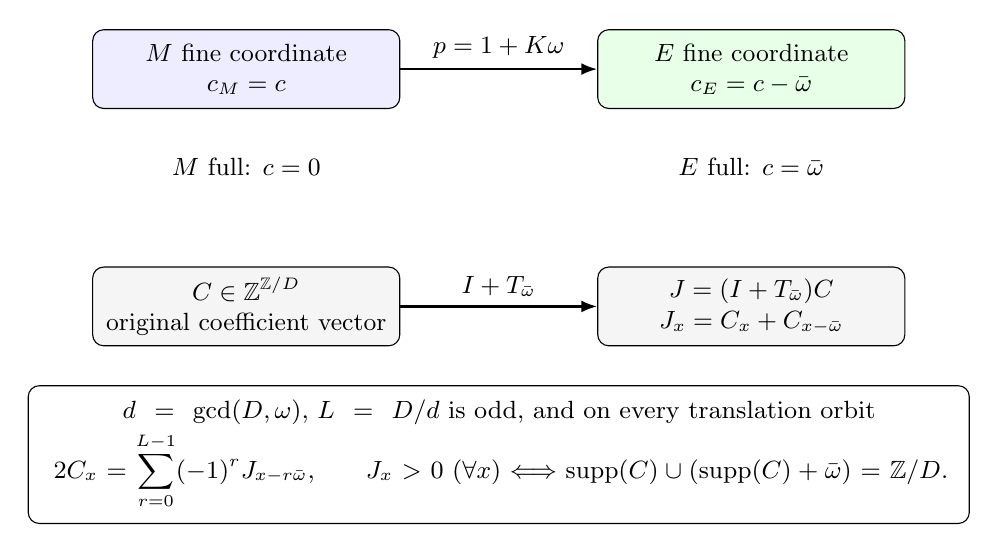
\begin{tikzpicture}[
  font=\small,
  box/.style={draw,rounded corners,minimum height=10mm,minimum width=39mm,align=center},
  map/.style={-{Latex[length=2mm]},thick}
]
\node[box,fill=blue!7] (m) {$M$ fine coordinate\\$c_M=c$};
\node[box,fill=green!9,right=25mm of m] (e) {$E$ fine coordinate\\$c_E=c-\bar\omega$};
\draw[map] (m) -- node[above] {$p=1+K\omega$} (e);
\node[below=5mm of m,align=center] {$M$ full: $c=0$};
\node[below=5mm of e,align=center] {$E$ full: $c=\bar\omega$};

\node[box,below=20mm of m,fill=black!4] (c)
  {$C\in\mathbb Z^{\mathbb Z/D}$\\original coefficient vector};
\node[box,right=25mm of c,fill=black!4] (j)
  {$J=(I+T_{\bar\omega})C$\\$J_x=C_x+C_{x-\bar\omega}$};
\draw[map] (c) -- node[above] {$I+T_{\bar\omega}$} (j);

\node[draw,rounded corners,below=10mm of $(c)!0.5!(j)$,align=center,
      text width=116mm,inner sep=5pt] (inverse)
  {$d=\gcd(D,\omega)$, $L=D/d$ is odd, and on every translation orbit\\[2pt]
   $\displaystyle 2C_x=\sum_{r=0}^{L-1}(-1)^rJ_{x-r\bar\omega}$,\qquad
   $\displaystyle J_x>0\ (\forall x)\Longleftrightarrow
   \operatorname{supp}(C)\cup
   (\operatorname{supp}(C)+\bar\omega)=\mathbb Z/D$.};
\end{tikzpicture}

\caption{Exact common-trace channel shift and odd-orbit inverse.}
\end{figure}

\begin{theorem}[Mixed-order bounded section]
Choose distinct indices $i_1,\ldots,i_k$, and let
$g_0=D$, $g_j=\gcd(g_{j-1},\lambda_{i_j})$, $m_j=g_{j-1}/g_j$.
Suppose $g_0>\cdots>g_k=1$ and $N_{i_j}\ge m_j$. Then
\[
 C_x\ge(\prod_{i\notin I}N_i)
          \prod_j\lfloor N_{i_j}/m_j\rfloor>0\quad(x\in\mathbb Z/D).       \tag{6}
\]
The $D$ bounded digits $0\le t_{i_j}<m_j$ give a bijection with $\mathbb Z/D$.
The empty chain for $D=1$ is included. If all selected $N_{i_j}=m_j$, equality
holds in (6).
\end{theorem}
\begin{proof}
The image of $\lambda_{i_j}$ generates
$g_j\mathbb Z/D$ modulo $g_{j-1}\mathbb Z/D$, a cyclic quotient of order $m_j$.
For a residue $c_k=x$, invert backwards:
\[
 t_{i_j}=(c_j/g_j)(\lambda_{i_j}/g_j)^{-1}\pmod{m_j},\quad
 0\le t_{i_j}<m_j,\quad c_{j-1}=c_j-\lambda_{i_j}t_{i_j}\pmod D.          \tag{7}
\]
The remaining residue is divisible by $g_{j-1}$, ending in zero. Each quotient
forces its unique digit. Partition each selected interval into full blocks of
size $m_j$. Every choice of blocks and of other coordinates translates the
required residue and gives one distinct original word by (7), proving (6).
\end{proof}

\begin{theorem}[Partial-chain quotient criterion]
Allow the chain to stop at $g=g_k>1$. Put
\[
 B=\prod_j\lfloor N_{i_j}/m_j\rfloor,
 \qquad
 Q_y=\#\{(t_i)_{i\notin I}:\sum_{i\notin I}\lambda_it_i\equiv y\pmod g\}.
\]
Then
\[
 C_x=BQ_{x\bmod g}+E_x,\qquad E_x\ge0,                         \tag{8}
\]
with every $E_x=0$ if $m_j\mid N_{i_j}$ for all selected coordinates. For the
common channels of Theorem~\ref{thm:short-affine}, with
$\delta=\omega\pmod g$,
\[
 C_x+C_{x-\bar\omega}
 \ge B(Q_{x\bmod g}+Q_{(x\bmod g)-\delta}).                    \tag{9}
\]
It follows that the complete-block subsource isolated by this partial chain
forces all two-channel targets exactly when
\[
 \operatorname{supp}(Q)+\{0,\delta\}=\mathbb Z/g.              \tag{10}
\]
If $d_g=\gcd(g,\delta)$, condition (10) requires the sharp lower bound
$|\operatorname{supp}(Q)|\ge(g+d_g)/2$. If the gcd of $g$ with all residual
steps is greater than one, (10) is impossible.
\end{theorem}
\begin{proof}
Retain every complete radix block in each selected interval. A fixed tuple of
block offsets lies in $g\mathbb Z/D$, and the within-block decoder is a
bijection onto that subgroup. Each residual tuple whose sum is $x$ modulo $g$
therefore gives one word over every one of the $B$ block tuples. Words meeting
a terminal interval form $E_x\ge0$, proving (8) and its equality case. Formula
(9) is (8) at the two exact channel targets. Formula (10) follows because all
coefficients are nonnegative. Its support bound is the odd-cycle argument from
Theorem~\ref{thm:short-affine}. If all residual sums lie in a proper subgroup
$b\mathbb Z/g$, the complete-block support and one translate meet at most two
of its $b\ge3$ cosets, so they cannot cover $\mathbb Z/g$. Terminal intervals
remain in the original coefficient vector and may add further words.
\end{proof}

The digit set is not given the wrong product-group law: in $\mathbb Z/9$ with
steps $(6,1)$ and radices $(3,3)$, the actual carry is
$(0,2)\star(0,1)=(2,0)$, not $(0,0)$. The exact multiplicity is also retained.
In the equality case every bin has $\mu=\prod_{i\notin I}N_i$ original words;
the free-integer coefficient kernel has rank $D(\mu-1)$. After choosing one
reference word in each residue fibre, its differences from the other words in
that fibre form a basis. The decoder inverts the augmented residue-and-unused-
digit map; the residue projection alone has $\mu$-point fibres.

\begin{figure}[ht]
\centering
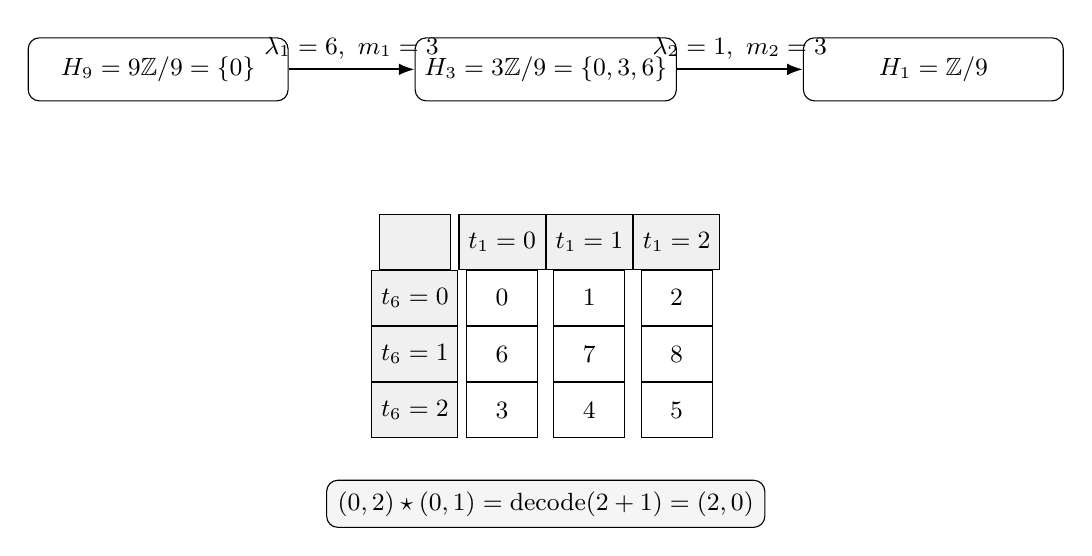
\begin{tikzpicture}[
  font=\small,
  chain/.style={draw,rounded corners,minimum width=33mm,minimum height=8mm,align=center},
  every edge/.style={draw,-{Latex[length=2mm]},thick}
]
\node[chain] (h9) {$H_9=9\mathbb Z/9=\{0\}$};
\node[chain,right=16mm of h9] (h3) {$H_3=3\mathbb Z/9=\{0,3,6\}$};
\node[chain,right=16mm of h3] (h1) {$H_1=\mathbb Z/9$};
\path (h9) edge node[above] {$\lambda_1=6,\ m_1=3$} (h3)
      (h3) edge node[above] {$\lambda_2=1,\ m_2=3$} (h1);

\matrix[below=13mm of h3,matrix of math nodes,
  nodes={draw,minimum width=9mm,minimum height=7mm,anchor=center},
  row 1/.style={nodes={fill=black!6}},
  column 1/.style={nodes={fill=black!6}}] (grid) {
  {} & t_1=0 & t_1=1 & t_1=2 \\
  t_6=0 & 0 & 1 & 2 \\
  t_6=1 & 6 & 7 & 8 \\
  t_6=2 & 3 & 4 & 5 \\
};
\node[below=4mm of grid,draw,rounded corners,fill=black!4,inner sep=4pt]
  {$ (0,2)\star(0,1)=\operatorname{decode}(2+1)=(2,0)$};
\end{tikzpicture}

\caption{The $9\to3\to1$ subgroup chain, exact residue section and nontrivial
carry.}
\end{figure}

All possible chain lower bounds can be optimized on a divisor DAG: use
$g\to\gcd(g,\lambda_i)<g$ when $N_i$ is at least the quotient order, with
edge weight $\lfloor N_i/m\rfloor/N_i$. Multiply the maximal path product by
$\prod_iN_i$. An effective coordinate cannot recur because every later gcd
already divides its step. Thus at most $n\tau(D)$ candidate edges suffice.
Failure of this test is not absence of the target coefficient.

\paragraph{Arithmetic beyond unit directions.}
For
\[
 R=243,\quad a=H\cdot53\cdot163\cdot271,\quad p=4a-R,\quad H\equiv29\pmod{210},
\]
retain the actual M packet with centred exponents $\{-1,1\},[-1,1],[-1,1]$
at the three displayed primes, all other centred exponents zero. It has
\[
 \mathcal C=(1+X^5)(1+X^6+X^{12})(1+X+X^2)
           =2\sum_{i=0}^8X^i\pmod{X^9-1}.
\]
The chain $9\to3\to1$ has radices $3,3$. The previous total unit width is only
three, below eight. One original M return is
$(h,r,s,\lambda)=(H,44173,53,182)$.

For
\[
 R=675,\quad a=H\cdot89\cdot271^2\cdot1801,\quad p=4a-R,
 \quad H\equiv101\pmod{210},
\]
use centred exponents $\{-1,1\},[-2,2],[-1,1]$. Now
\[
 \mathcal C=(1+X^{11})\left(\sum_{j=0}^4X^{6j}\right)
                    (1+X^{10}+X^{20})
 =2\sum_{i=0}^{14}X^i\pmod{X^{15}-1}.
\]
Both selected steps $6,10$ are nonunits; their radices are $5,3$.
The only unit width is one. An original M return is
$(H,1801,6536249,9686)$.
Each displayed $p$-family is a reduced linear progression modulo $840A$, where
$A$ is the displayed fixed product. Modulo its prime factors, $p=-R$ is a unit;
modulo $840$, $p=1$. Dirichlet supplies infinitely many prime members [2].
No arbitrary-prime coverage is inferred.

The last capacity bound is arithmetically necessary for uniform completion.
For an odd defect $D$, fix a strict chain
$g_0=D$, $g_j=\gcd(g_{j-1},\lambda_j)$, $g_k=1$, and put
$m_j=g_{j-1}/g_j$, $m=m_k$, $R=3D^2$, $K=3D$. Realize earlier steps by primes
$q_i=1+K\lambda_i\pmod R$ with exponents $(m_i-1)/2$. For the last step choose
$q_k=-1+Kc\pmod R$, $2c=-\lambda_k\pmod D$, with exponent $m-1$.
Since $K^2=3R$,
\[
 q_k^2\equiv1-2Kc\pmod R,\qquad (q_k^2-1)/K\equiv\lambda_k\pmod D.
\]
For the earlier centred exponents and the odd last exponents,
\[
 z\equiv-1+K\left(c\beta_k-\sum_{i<k}\lambda_i\beta_i\right)\pmod R.
\]
The earlier exact-radix intervals biject onto $H_m=m\mathbb Z/D$. The last
$m-1$ exponents, multiplied by the unit $c\pmod m$, give every nonzero quotient
class and no zero. The exact fine count is zero on $H_m$ and one elsewhere,
with stabilizer exactly $H_m$. The CRT conditions
$p=1\pmod{840}$, $p=4A-R\pmod{4A^2}$ are compatible and reduced, proving
infinitely many hard-prime original packets with that defect. Other source
words are retained; this does not furnish or claim a conjectural counterexample.

The separate finite realization is
\[
 D=9,\quad(q_1,q_2)=(163,107),\quad H=523,\quad
 a=976015801,\quad p=3904062961,
\]
with coefficient vector $(0,1,1,0,1,1,0,1,1)$ and stabilizer
$\{0,3,6\}$. Its exact-exponent progression is
$p=3904062961+2925429291933960t$. The displayed $R=243$ shell is empty, but
the same prime has the full E witness
$(a_0,R_0,u_0)=(976015741,3,89)$, so this is not an ES counterexample.

\begin{theorem}[A labelled upward factor exchange]
For an original shell and chosen $s\mid a$, put
$C=R+s$ and $M=p+C=4a+s$. All cells with the same labelled invariant are
\[
 s'\mid M,\quad M/s'\equiv1\pmod4,\quad 0<C-s'<p,
\]
\[
 a'=(M-s')/4,\quad R'=C-s',\quad h'=(M/s'-1)/4.                       \tag{11}
\]
Such a cell gives an original unit-ray E state precisely when $R'\mid M$.
Then $u'=h'$, $r'=1$, $\kappa'=M/R'-1$, and its ordered denominators are
$(a',h's'\kappa',ph'\kappa')$.
\end{theorem}
\begin{proof}
The congruence is precisely the integral factorization $a'=h's'$ and implies
$R'\equiv3\pmod4$. The range gives the original first-half domain. Since
$s'\mid a'<p$, one has
$\gcd(R',s')=\gcd(4h's'-p,s')=\gcd(p,s')=1$. Thus the original E gate
$R'\mid4h'+1$ is equivalent to $R'\mid M=(4h'+1)s'$. Equivalently,
$p+s'=M-R'$, so $R'\mid p+s'$ is exactly $R'\mid M$.
Retaining $s,s'$ inverts (11), with $a'-a=(s-s')/4$.
\end{proof}

At $p=67369$, the proper trace $(a,R,u,h,r,s)=(16849,27,4067,83,7,29)$
has $C=56$, $M=67425$. Taking $s'=25$, $R'=31$ gives $a'=16850$, $h'=674$,
$\kappa'=2174$ and
\[
 \frac4{67369}=\frac1{16850}+\frac1{36631900}+\frac1{98714178844}.
\]

\begin{figure}[ht]
\centering
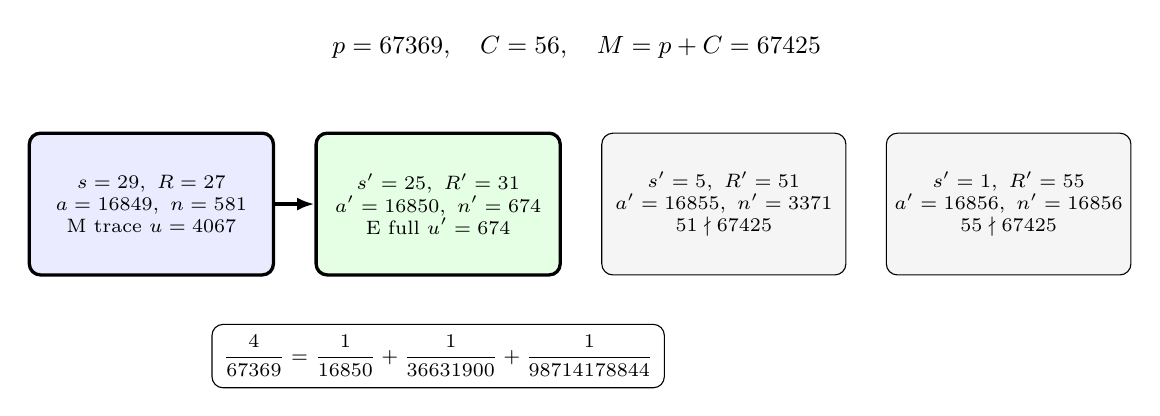
\begin{tikzpicture}[
  font=\scriptsize,
  cell/.style={draw,rounded corners,align=center,minimum width=31mm,minimum height=18mm,inner sep=3pt},
  source/.style={cell,fill=blue!8,very thick},
  target/.style={cell,fill=green!10,very thick},
  fail/.style={cell,fill=black!4},
  arrow/.style={-{Latex[length=2.2mm]},very thick}
]
\node[font=\small] (head) {$p=67369,\quad C=56,\quad M=p+C=67425$};
\node[source,below=8mm of head,xshift=-54mm] (c1)
  {$s=29,\ R=27$\\$a=16849,\ n=581$\\M trace $u=4067$};
\node[target,right=5mm of c1] (c2)
  {$s'=25,\ R'=31$\\$a'=16850,\ n'=674$\\E full $u'=674$};
\node[fail,right=5mm of c2] (c3)
  {$s'=5,\ R'=51$\\$a'=16855,\ n'=3371$\\$51\nmid67425$};
\node[fail,right=5mm of c3] (c4)
  {$s'=1,\ R'=55$\\$a'=16856,\ n'=16856$\\$55\nmid67425$};
\draw[arrow] (c1) -- (c2);
\node[draw,rounded corners,below=6mm of c2,inner sep=4pt,align=center]
  {$\displaystyle\frac4{67369}=\frac1{16850}+\frac1{36631900}
       +\frac1{98714178844}$};
\end{tikzpicture}

\caption{All four cells in the $p=67369$, $C=56$ fibre and the exact selected
upward arrow.}
\end{figure}

Every earlier shell is fully exhausted in the certificate and has no integer
gate. The return must increase $a$ at this input. More generally, set
$h=83+4650k$, $p=812h-27=67369+3775800k$. On every prime member, the same
proper trace $(203h,27,49h)$ returns to
\[
 a'=203h+1,\ R'=31,\ h'=(203h+1)/25,\ r'=1,\ s'=25,\ \kappa'=(p+25)/31.
\]
All divisions are exact and the prime progression is reduced. The previous
word/ray deletions and factor-sum return fail on that marked source. No assertion
that every old shell is wholly empty along this progression is needed.

At $p=97,a=40,u=2$ in M, the invariant instead has $C=83,M=180$. Its entire
cell list is $(a',R',s')=(36,47,36),(40,63,20),(44,79,4)$, each with both full
gates empty. Thus a fixed invariant fibre need not be occupied. Universal
existence still requires an argument linking original sources across shells;
neither theorem assumes that missing first source.

\paragraph{Complete incoming source, rather than an unmarked inverse.}
For a supplied primitive target with $r'=1$, recover $C=R'+s'$ and
$M=p+C$. Enumerate every cell in (11). For each cell enumerate $r\mid n$
with $\gcd(r,s)=1$ and set
\[
 h=n/r,\qquad u=nr,\qquad a=ns.
\]
The E and M source tests are respectively
\[
 R\mid(pr+s)^2,\qquad R\mid(r+s)^2.
\]
These finite tests are necessary and sufficient for all canonical trace inputs
whose retained $s$ produces this $C$. The factorization of the old shell gives
$n=hr$ and recovers exactly the displayed data; conversely the exact gcd factorization
of $a=ns,u=nr$ gives $(h,r,s)$ because $\gcd(r,s)=1$. An M word already
records its ordered tails. On ordered rational triples the exact E swap is
$\tau_E(a,Y,Z)=(a,Z,Y)$ with $\tau_E^2=\operatorname{id}$; it does not
generally preserve the original E word box and is not inserted into the
canonical incoming fibre.
The forward arrow records its chosen target; forgetting that choice gives a
relation whenever several terminal cells pass. The free-integer kernel of the
arrow projection has a basis formed by choosing one reference arrow in each
target fibre and subtracting it from every other arrow in that fibre. It is not
a quotient that identifies the old and new factor supports.

For the target at $p=67369$, the complete cells have $(R,s)$ equal to
\[
 (27,29),\ (31,25),\ (51,5),\ (55,1).
\]
Only $(31,25)$ is an exterior terminal cell. Its canonical incoming trace fibre
contains precisely the original M word $4067$ at $a=16849$ and the full E word
$674$ at $a=16850$. Thus the source-changing arrow crosses the obstruction;
its complete fibre does not assert that a corresponding arrow exists at every
prime. At $p=97$ the three cells given above have no full original gate even
when all their words, not just the unit-ray words, are tested.

\paragraph{Evidence.}
The accompanying full source gives every inverse fibre and finite bound.
The standard-library checks compare the complete original boxes through the
declared prime bound and exhaust 161887 additive polynomials, with a separate
subsequence-based optimum check and independent primitive-state enumeration.
The files distinguish observed runs, finite example searches and written
universal proofs. No human review, Lean build or priority determination is claimed.

\begin{thebibliography}{9}
\bibitem{1} Elsholtz, C., \& Tao, T. (2013). Counting the number of solutions to
the Erd\H{o}s--Straus equation on unit fractions. \emph{J. Aust. Math. Soc., 94},
50--105. \href{https://arxiv.org/abs/1107.1010}{arXiv:1107.1010}, \S2.
\bibitem{2} Sutherland, A. V. (2017). \emph{Dirichlet's theorem on primes in
arithmetic progressions}. MIT 18.785 Lecture 18, Theorem 18.1.
\href{https://math.mit.edu/classes/18.785/2017fa/LectureNotes18.pdf}{Lecture notes}.
\bibitem{3} Lopez, M. A. (2024). \emph{A Complete Congruence System for the
Erdos--Straus Conjecture}. \href{https://arxiv.org/abs/2404.01508}{arXiv:2404.01508}.
Introduction and Type~A/B definitions.
\end{thebibliography}
\end{document}
